\documentclass[main.tex]{subfiles}

\begin{document}

\section{Multiple option}
Read the following quastions and identify the option that best answer each, then write its letter on the line.

\paragraph{1} The range of the function $f(x)=\exp\qty[ax]-b$ is

\begin{enumerate*}
    \item $f(x)\in\qty(b,\infty)\quad$
    \item $f(x)\in[b,\infty)\quad$
    \item $f(x)\in[-b,\infty)\quad$
    \item $f(x)\in\qty(-b,\infty)\quad$
\end{enumerate*}

\paragraph{2} The graph of the function $f(x)=a^x$ when $x$ goes to infinity $x\to\infty$ goes to:

\begin{enumerate}
    \item The function goes to minus infinity $f(x)\to-\infty\quad$
    \item The function goes to plus infinity $f(x)\to\infty\quad$
    \item The function goes to zero $f(x)\to 0\quad$
    \item The function goes to the base $a$ $f(x)\to a\quad$
\end{enumerate}

\paragraph{3} Which of the following equations show a logarithmic function base $a$ with a translation fo $n$ units left and $m$ units down and tends to minus infinity $f(x)\to-\infty$ when the domain tends to $n$ ($x\to n$).

\begin{enumerate*}
    \item $f(x)=\log_a(x+n)+m\quad$
    \item $f(x)=\log_a(x+n)-m$ \\\\
    \item $f(x)=-\log_a(x-n)+m\quad$
    \item $f(x)=-\log_a(x-n)-m\quad$
\end{enumerate*}

\paragraph{4} Which of the following statements represent the "Logarithm of a Product"

\begin{enumerate*}
    \item $\log_a(M)+\log_a(N) = \log_a(MN)\quad$
    \item $P\log_a(M)=\log_a(M^P)$ \\\\
    \item $\log_a(M)-\log_a(N)=\log_a(\frac{M}{N})\quad$
    \item $-\log_a(M)=\log_a(\frac{1}{M})\quad$
\end{enumerate*}

\paragraph{5} The domain of the function $f(x)=\log_a(x)-m$ is

\begin{enumerate*}
    \item $x\in\qty(m,\infty)\quad$
    \item $x\in[m,\infty)\quad$
    \item $x\in[0,\infty)\quad$
    \item $x\in\qty(0,\infty)\quad$
\end{enumerate*}

%\paragraph{6} Which of the following graphs represents an exponential decay?

%\begin{figure}[ht!]
%    \centering
%    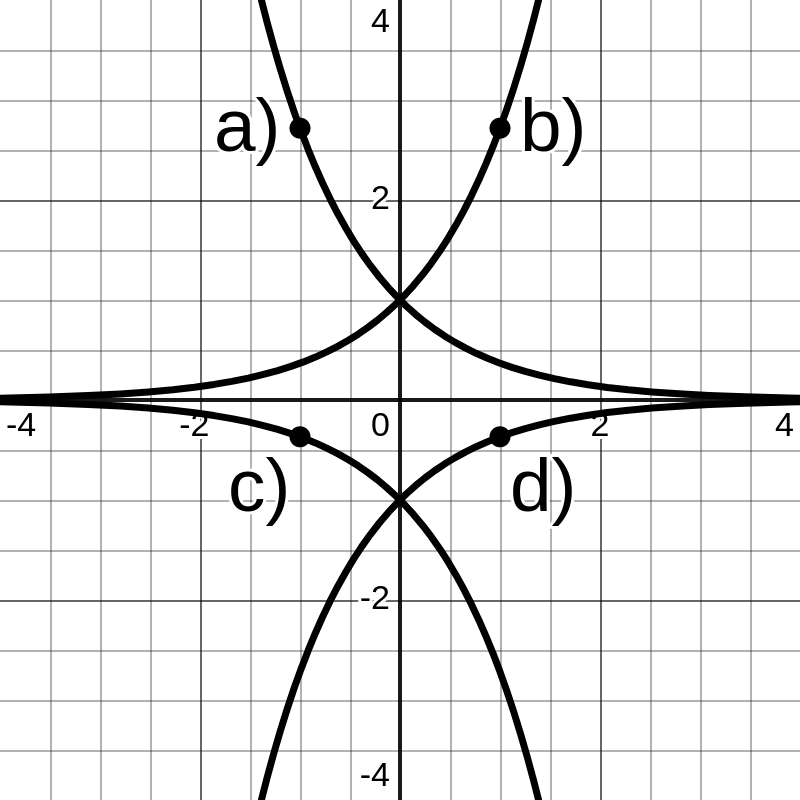
\includegraphics[width=0.45\textwidth]{../imgs/exp-log/exponentials.png}
%\end{figure}

\section{Algebra skills}
Answer the following exercises. frame or highlight yor final answer.

\paragraph{7} solve the following expressions for $x$.
Include your procedures in an external paper.
\begin{gather*}
    \log_a(mx) = c,\quad e^{x/d}=g
\end{gather*}

\section{Exponential and logarithmic equations}
Solve the following exercies in an orderly and clear manner.
Underline or frame your final answer.
Include the WHOLE procedure.
This is evidence for your answers, missing procedures will render the answer invalid.

\paragraph{8} Write and use the change of base formula to compute the folowing $\log_2\qty(\frac{1}{e})$  and report the numeric value with 6 decimals (Express the final answer in natural logarithm) .

\paragraph{9} Use the Laws of logarithms to expand the following expression, $ \log_e\qty(\frac{a^nb^m}{c^l}) $

\paragraph{10} Use the properties of logarithms to condense the following expression $ \log\qty[\frac{\ln(x^n)}{a\ln(x)}-b\ln(x)] $.

\paragraph{11} Determine the asymptote for the following function $ f(x)=a\qty(e^x-\frac{1}{b})+c(e^x+1) $

\paragraph{12} Find the intersection point between the line $f(x)=3$ and the following function $ f(x)=\log_a(x-m) + \log_b(x+n) $.

\paragraph{13} Find a function $m(t) = m_o e^{-rt}$ that models the amount of krypton-91 remaining in a canister after $t$ seconds.
Considering that at time $t=0$ the canister contains $3$ grams of this radioactive gas and that the half-life of krypton-91 is $10$ seconds ($m(10)=m_o/2$).


\end{document}

